\documentclass[a4paper,10pt, fleqn]{article}
\usepackage{graphicx} %Paquete para ingresar gráficos.
\usepackage{hyperref}
\usepackage{fancybox}
\usepackage[spanish]{babel} % Para división en sílabas español.
\usepackage[utf8]{inputenc} % Para poner acentos.
\usepackage{placeins} % Para poder usar \FloatBarrier para que las tablas e imagenes no se vayan de la seccion
\usepackage{float} % Para usar [H] en tablas e imagenes


%Encabezado y Pié de página
\usepackage{fancyhdr} %Paquete para encabezados y pie de página
\pagestyle{fancy} %Sin esta línea no se imprimiría el encabezado en todas las páginas

\fancyhf{} %Borra el encabezado anterior (Por defecto escribe el títutlo de la sección en la que se encuentra la hoja
\setlength{\headheight}{22.55pt}
\fancyhead[L]{
	{\textsf{Facultad de Ingeniería de la Universidad de Buenos Aires \\ 66.20 - Organización de Computadoras}}
}

\fancyhead[R]{\thepage}

\renewcommand{\footrulewidth}{0.4pt} %Ajusta el tamaño de las líneas separadoras en el pié de página
\renewcommand{\headrulewidth}{0.4pt} %Ajusta el tamaño de las líneas separadoras en el encabezado

\fancyfoot[L]{
	{\textsf{TP N$^{\circ}$0: Infraestructura Básica}} \\
}


%Carátula del Trabajo
\title{ \author{} %Lo pongo para que el warning no moleste :p
\setlength{\unitlength}{1cm} %Especifica la unidad de trabajo
\thispagestyle{empty}
\begin{picture}(18,0)
\put(0,0){
\includegraphics[width=1.5cm, height=3cm]{Logo1.png}}
\put(10.5,0){
\includegraphics[width=3cm, height=3cm]{Logo2.png}}
\end{picture}
\\[1.5cm]
\begin{center}
	\textbf{{\Huge Facultad de Ingeniería \\ Universidad de Buenos Aires}}\\[2cm]
	{ 66.20 Organización de Computadoras}\\[0.5cm]
	{ Trabajo Práctico N${^\circ}$0 : Infraestructura Básica}\\[2.5cm]
\end{center}

\begin{flushleft}
	\textbf{Integrantes:} \\[1cm]

 	\begin{tabular}{|c|c|}
		\hline
		\textbf{Padrón} & \textbf{Nombre} \\		
		\hline
		76187 & Lucas Hemmingsen  \\

	\end{tabular}
\end{flushleft}
\date{} %Hace que no se imprima la fecha en la cual se compilo el .tex
 }

\begin{document}
\maketitle %Hace que el título anterior sea el principal del documento
\newpage

\tableofcontents %Esta línea genera un indice a partir de las secciones y subsecciones creadas en el documento
\newpage

\section{Objetivos}
	El objetivo del presente trabajo consiste en familiarizarnos con las herramientas con las cuales se trabajará en el transcurso de la cursada. Las mismas son:
	\begin{itemize}
	  \item Compilador GCC
	  \item Shell de Unix
	  \item Emulador GXEmul
	  \item Sistema de Composición \LaTeX{}
	\end{itemize}
	\vspace{1cm}
 
\section{Introducción Teórica}
  \label{sec:InfoTeo}
  Para poner en práctica las herramientas citadas, el presente TP consiste en realizar un programa en lenguaje C que codifique información 
  un conjunto arbitrario de bytes en un conjunto formado por caracteres ASCII utilizando el esquema de codificación \emph{Base 64}
  A continuación se explican brevemente los conceptos y herramientas utilizadas necesarias para llevar a cabo esta tarea:

  \vspace{0.5cm}
	\subsection{Shell de Unix}
	  Un shell es un programa intérprete de comandos. Los comandos utilizados en el presente trabajo
	  son los siguientes:
		\begin{itemize}
		  \item \textbf{\emph{pipe}}: Toma lo que se encuentra a la izquierda del pipe como la salida estándar (\emph{stdout}) por defecto y lo pasa como
		      entrada estándar (\emph{stdin}) a lo que se este a la derecha del pipe. Puede servir para pasarle a un programa un
		      archivo y que este lo reciba por la entrada estándar
		  \item \textbf{echo}: Imprime un texto en \emph{stdout}.
		  \item \textbf{cat}: Con este comando se pueden ver, así como también concatenar, varios archivos. 
		    Escribe en la salida estándar.
		\end{itemize}
		\vspace{0.5cm}

	\subsection{Compilador GCC}
		GCC es un compilador gratuito, Open Source y multiplataforma que permite compilar código C. 
		El mismo es un compilador estándar, es decir, que respeta la norma ISOC99 o ANSI dependiendo de su versión, por lo cual se utilizan las 
		bibliotecas estándar para trabajar con el mismo. En esta asignatura el mismo es de gran utilidad dado que permite tener acceso  al código 
		\emph{assembly} equivalente a nuestro programa en C. A continuación se detallan brevemente algunos parámetros que podemos darle al GCC:
		\begin{itemize}
			\item \textbf{-Wall:} Activa todos los warnings.
			\item \textbf{-o file} Almacena la salida del programa en un archivo (\emph{en este caso en file})
			\item \textbf{-O0:} Desactiva las optimizaciones
			\item \textbf{-O3:} Activa todas las optimizaciones
			\item \textbf{-g:} Genera código agregando líneas para el \emph{debbugger}
			\item \textbf{-S:} Detiene el compilador luego de generar el código \emph{assembly}
			\item \textbf{-mrnames(solo para MIPS):} Indica al compilador que genera la salida utilizando 
									 nombre de registro en lugar de número de registro
		\end{itemize}
		Para generar el archivo ``main.s'' con el código \emph{assembly} se debe ejecutar el siguiente comando: 
		  \begin{verbatim}
			      gcc -Wall -O0 -S -mrnames main.c
		  \end{verbatim}
		Para compilar el código se debe ejecutar el siguiente comando:
		\begin{verbatim}
			      gcc -Wall -O0 -o tp0 main.c
		 \end{verbatim}
		\vspace{0.5cm}

	\subsection{Emulador GXEmul}
		Es un emulador gratuito y Open Source de la arquitectura de computadores MIPS. Tiene como ventajas que puede correr algunos sistemas operativos
		sin modificaciones (especialmente \emph{netBSD}), su portabilidad y velocidad de emulación dado que realiza la traducción binaria en 
		tiempo real. 
		\vspace{0.5cm}
	
					
\section{Desarrollo}
	A partir de los conceptos teóricos desarrollados en la sección anterior (\ref{sec:InfoTeo}) se procedió a crear un programa en 
	C que pudiese codificar información mediante el esquema de codificación \emph{Base64} a partir de una muestra:
	\vspace{0.5cm}

	\subsection{Modo de Operación}
                Para compilar la aplicación hay que posicionarse en el directorio en el que se encuentra el archivo ``tp0.c'', y ejecutar el siguiente comando:
                \begin{verbatim}
                  gcc -Wall -O0 -o tp0 tp0.c
                \end{verbatim}
 
		La aplicación desarrollada debe recibir ya sea por entrada estándar o mediante archivos de entrada, una muestra de N bytes. 

		\begin{itemize}
			\item \textbf{-e --encode:} Por medio de este comando se indica que el algoritmo debe codificar la información pasada a \emph{Base64}.
			\item \textbf{-d --decode:} Por medio de este comando se indica que el algoritmo debe decodificar la información pasada desde \emph{Base64}.
			\item \textbf{-i --input file:} Por medio de este comando se indica el archivo de entrada para realizar la codificación o decodificación. En caso de no indicar un archivo de entrada, el programa tomará la entrada de \emph{stdin}.
			\item \textbf{-o --output file:} Por medio de este comando se indica el archivo de salida para realizar la codificación o decodificación. En caso de no indicar un archivo de salida, el programa escribirá la salida en \emph{stdout}.
			\item \textbf{-h --help:} Despliega la ayuda.
			\item \textbf{-v --version:} Muestra la versión.
		\end{itemize} 
		
		\vspace{0.5cm}
	
	\subsection{Ejemplos}
	     Primero, usamos la opcion -h para ver el mensaje de ayuda:
	     \begin{verbatim}
		$tp0 -h
		OPTIONS:
		-e --encode Encodes to Base64
		-d --decode Decodes from Base64
		-i --input file Reads from file or stdin
		-o --output file Writes to file or stdout
		-v --version Show version string
		-h --help Print this message and quit

 	     \end{verbatim}
	     
	     Si quisieramos codificar y decodificar el arreglo de bytes "foo" debemos ejecutar:
             \begin{verbatim}
                $echo -n "foo" | tp0 -e | tp0 -d
				foo
             \end{verbatim}
			 Lo que hace esta línea es tomar el arreglo de bytes "foo" como entrada del programa para codificar, tomándolo desde la entrada estándar,
			 codifica la información a \emph{Base64} y escribe la salida por la salida estándar, para luego tomar esta salida 
			 como entrada estándar para decodificar la información, escribiendo la salida por salida estándar, siendo "foo" esta salida.
	    Si se está codificando información y luego se desea ver la salida codificada, es recomendable especificar un archivo de salida y luego para visualizar el contenido del archivo binario en formato hexadecimal y separado en bytes, utilizar el comando \emph{hexdump}:
		\begin{verbatim}
		$echo -n "foo" | tpo -e -o foo.txt
		\end{verbatim}	    

             \begin{verbatim}
                hexdump -C foo.txt
             \end{verbatim}
	      De cualquier manera, si se especifica un archivo, este puede verse con cualquier editor 
	      de texto, o por consola con el comando
             \begin{verbatim}
                cat foo.txt
             \end{verbatim}
 

\section{Implementación}
	\subsection{Determinaciones Previas}
	  \begin{itemize}
			\item Siempre que se ingrese el parámetro de ayuda (-h o \---help) junto con cualquier otro, se ignorará este último. 
			      Por ejemplo ``echo ``abc'' ./tp0 -h'' sólo muestra el mensaje de ayuda.
			\item Si no se especifica codificar (-e) o decodificar (-d) el programa mostrará el menú de ayuda y finalizará la ejecución.
			\item Si alguno de los archivos pasados por parámetro no puede ser leído, la ejecución termina mostrando el error por stderr.
			\item Si se selecciona codificar y decodificar no se ejecutará la sentencia y mostrará el menú de ayuda.
			\item Si se ingresan archivos a través de los argumentos y además alguno por stdin, solo se tendrán en cuenta los primeros, ignorando
			      el ingresado por entrada estándar.
			\item Si al decodificar la información se obtiene algún caracter invalido el programa mostrará un error por stderr y finalizará.
	  \end{itemize}
	

	\subsection{Código Fuente}

\begin{Verbatim}[fontsize=\tiny]

#include <stdio.h>
#include <stdlib.h>
#include <getopt.h>

#define ALPHABET "ABCDEFGHIJKLMNOPQRSTUVWXYZabcdefghijklmnopqrstuvwxyz0123456789+/"
#define ALPHABET_LENGTH 64
#define ENDING_CHAR '='
#define ENDING_CHAR_INT 61
#define ENCODE_SIZE 6
#define DECODE_SIZE 8
#define BUFFERSIZE 12

void error()
{
	fprintf(stderr, "Error al decodificar\n");
	exit(EXIT_FAILURE);
}

int indexOf(char aChar){
	int i;
	for(i= 0;i < ALPHABET_LENGTH;i++){
		char alph_char = ALPHABET[i];
		if(alph_char == aChar)
			return i;
	}
	error();
	return -1;
}

int count = 0;
int acum = 0;
int length = 0;

void doEncode(int value)
{
	acum = (acum << 1) | value;
	count++;
	if(count == ENCODE_SIZE){		
		++length;
		putc((int)ALPHABET[acum], stdout);
		count = 0;
		acum = 0;
	}
}

void encode64(char * const input, size_t amount)
{
	int i,j;

	for (i = 0; i< amount; i++)
	{
		char aChar =  input[i];
		for (j = DECODE_SIZE -1 ; j >=0 ; --j)
			doEncode(((aChar >> j) & 0x01));
	}
}

void doDecode(int value)
{
	acum = (acum << 1) | value;
	count++;
	if(count == DECODE_SIZE){		
		++length;
		putc(acum, stdout);
		count = 0;
		acum = 0;
	}
}

void decode64(char * const input, size_t amount)
{
	int i,j;
	char aChar;

	for (i = 0; i< amount && (input[i] != ENDING_CHAR); i++)
	{
		int index =  indexOf(input[i]);
		aChar =  index;
		for (j = ENCODE_SIZE - 1; j >= 0; j--)
			doDecode(((aChar >> j) & 0x01));
	}
}

void process(int encode, char* buffer, size_t amount)
{
	if (encode)
		encode64(buffer, amount);
	else
		decode64(buffer, amount);
}

void closeProcess(int encode)
{
	int i;
	if(encode)
	{
		if(count < ENCODE_SIZE && count > 0)
		{
			while(count != 0)
			{
				doEncode(0);
			}

			for (i = 0; i < 4 - length % 4; i++)
				putc(ENDING_CHAR_INT, stdout);
		}
	}
	fflush(stdout);
}

void openInFile(char * file){
	FILE * ifp = freopen(file, "rb", stdin);
	if (ifp == NULL) {
	  fprintf(stderr, "Can't open input file\n");
	  exit(EXIT_FAILURE);
	}
}

void openOutFile(char * file){
	FILE * ofp = freopen(file, "wb", stdout);
	if (ofp == NULL) {
	  fprintf(stderr, "Can't open output file\n");
	  exit(EXIT_FAILURE);
	}
}

void print_help(){
	fprintf(stdout, "Modo de empleo: ./tp0 [OPTIONS]\n"
"OPTIONS:\n"
"-e --encode Encodes to Base64\n"
"-d --decode Decodes from Base64\n"
"-i --input file Reads from file or stdin\n"
"-o --output file Writes to file or stdout\n"
"-v --version Show version string\n"
"-h --help Print this message and quit\n");
}

void print_version(){
	fprintf(stdout, "Version 1.0\n");
}

void selectionError() {
	fprintf(stderr, "Error: decode and encode selected.\n");
	print_help();
	exit(EXIT_FAILURE);
}
int main(int argc,  char* const* argv)
{
	int encode = -1;
	int c;
	extern char *optarg;
	extern int optind, opterr, optopt;
	/* Una cadena que lista las opciones cortas válidas */
	const char* const opcionesCortas = "edi:o:vh";

	/* Una estructura de varios arrays describiendo las opciones largas */
	const struct option opcionesLargas[] = {
	  { "help",	  no_argument, NULL,'h'},
	  { "version", no_argument, NULL,'v'},
	  { "input",no_argument, NULL,'i'},
	  { "output",no_argument, NULL,'o'},
	  { "encode",no_argument, NULL,'e'},
	  { "decode",no_argument, NULL,'d'},
	  { NULL,     no_argument, NULL, 0 }
	};

	opterr = 0;

	while ((c = getopt_long(argc, argv, opcionesCortas, opcionesLargas, NULL)) != -1)
	 switch (c)
	   {
	   case 'e':
	     if (encode == -1)
	    	 encode = 1;
	     else
	    	 selectionError();
	     break;
	   case 'd':
	     if (encode == -1)
	    	 encode = 0;
	     else
	    	 selectionError();
	     break;
	   case 'i':
	     openInFile(optarg);
	     break;
	   case 'o':
	     openOutFile(optarg);
	     break;
	   case 'h':
	     print_help();
	     exit(EXIT_SUCCESS);
	   case 'v':
	     print_version();
	     exit(EXIT_SUCCESS);
	   case '?':
	     if (optopt == 'i' || optopt == 'o')
	       fprintf (stderr, "Option -%c requires an argument.\n", optopt);
	     else
	       fprintf (stderr, "Unknown option character\n");
	     print_help();
	     exit(EXIT_FAILURE);
	   default:
	     abort ();
	   }

     /*************************************************************/

	char buffer[BUFFERSIZE];
	size_t amount;

	while (1) /* break with ^D or ^Z */
	{
		amount=fread(buffer, 1, BUFFERSIZE , stdin);
		process(encode, buffer, amount);
		if(feof(stdin))
			break;
	}

	closeProcess(encode);
	fclose (stdin);
	fclose (stdout);

	return 0;
}

\end{Verbatim}



\section{Pruebas}
      \begin{itemize}
      \item \textbf{Codificación y Decodificación trivial: }\\
      Si ejecutamos la siguiente secuencia de comandos en el shell:\\
      \begin{verbatim}
$ echo -n foo | ./tp0 -e | ./tp0 -d
foo
      \end{verbatim}
      Este caso demuestra que el programa al codificar y decodificar devuelve la misma información de entrada.\\
      Si ejecutamos la siguiente secuencia de comandos en el shell:\\
      \begin{verbatim}
$ echo -n foo | ./tp0 -e
Zm9v	
      \end{verbatim}
      nos devuelve la misma codificación que en el ejemplo del enunciado. \\
      Si ejecutamos la siguiente secuencia de comandos en el shell:\\
      \begin{verbatim}
$ echo -n Zm9v | ./tp0 -d
foo	
      \end{verbatim}
      volvemos a obtener la información pasada antes de codificarla. \\
      
      \item \textbf{Selección de un algoritmo por defecto: }\\
      En el caso de no explicitar la opción de codificación o decodificación, el programa por defecto codificará la información que se le pase.\\
      \begin{verbatim}
$ echo -n hola | ./tp0
aG9sYQ==
      \end{verbatim}


      \item \textbf{Caracteres fuera del alfabeto al decodificar: }\\
      Al decodificar, al pasarle como entrada caracteres que no se encuentran en el alfabeto, el programa indicará que hay un error al decodificar y detendrá la ejecución del mismo.
      \begin{verbatim}
$ echo -n **foo | ./tp0 -d
Error al decodificar
      \end{verbatim}

      
      \item \textbf{Selección de un archivo inexistente: }\\
      \begin{verbatim}
$ ./tp0 -e -i sdsd.txt
Can't open input file
      \end{verbatim}
      Si consideramos  que el archivo ``sdsd.txt'' no existe, nos saldrá por stderr una línea indicando el error. \\

      \item \textbf{Codificación y decodificación de un archivo binario: }\\
      Se generó un archivo binario de 2KB y se encriptó el mismo utilizando nuestro programa y utilizando el programa base64 incluido en el sistema operativo y se compararon ambas salidas.
      Luego se desencriptaron los datos encriptados y se comparó con el archivo original.\\
      \begin{verbatim}
$ dd if=/dev/urandom of=file.txt bs=2048 count=1
1+0 records in
1+0 records out
2048 bytes (2.0 kB) copied, 0.000291106 s, 7.0 MB/s
$ ./tp0 -e -i file.txt -o salida.txt
$ base64 -w0 file.txt > salidabase64.txt
$ diff salida.txt salidabase64.txt
$ ./tp0 -d -i salida.txt -o entrada.txt
$ diff file.txt entrada.txt
$
      \end{verbatim}

      \item \textbf{Script de pruebas: }\\
      En la realizacion de este trabajo práctico se utilizaron muchas pruebas en todas las etapas del desarrollo.
      Para facilitar las mismas se creó un script (adjunto en el presente trabajo) que realiza todas las pruebas automáticamente y entrega un informe 
      detallando los resultados de los mismos.
Para las pruebas realizadas en este trabajo se lo probó contra la versión del base64 instalada en el sistema operativo con la opcion -w0 para que no agrupe por líneas.\\
A continuación se muestra la salida de dicho sistema, a modo de ejemplo:\\

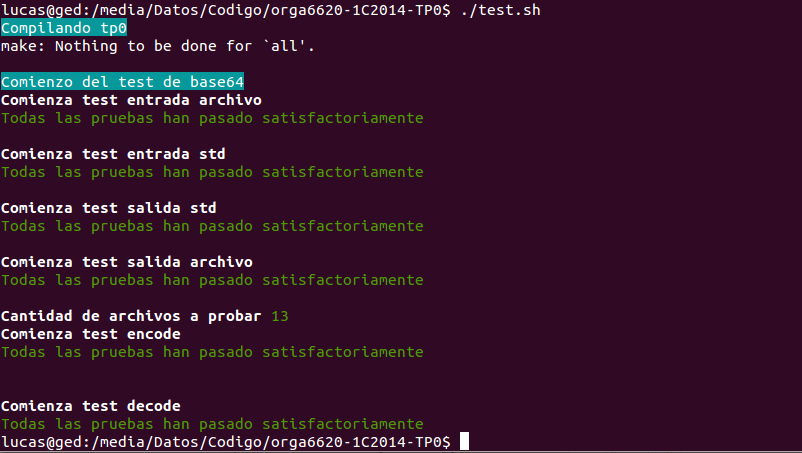
\includegraphics[width=0.9\textwidth]{tests.png}

El mismo prueba tanto los distintos modos de entrada y salida del ejecutable como también todos los casos de pruebas que se plantearon.
Los archivos de prueba que se utilizaron en el trabajo son los siguientes (archivos adjuntos en la carpeta tests):\\
\begin{itemize}

\item \textbf{vacio.test:} Archivo vacío con el objetivo probar el funcionamiento si no hay entrada.\\

\item \textbf{test\_1\_caracter:} Archivo con un sólo caracter con el objetivo de probar el funcionamiento con menos de 24 bytes.

\item \textbf{test\_2\_caracteres:} Archivo con dos caracteres con el objetivo de probar el funcionamiento con menos de 24 bytes.

\item \textbf{test\_2\_caracteres:} Archivo con 3 caracteres con el objetivo de probar el funcionamiento con 24 bytes.

\item \textbf{Otros archivos de distintos valores para probar los resultados:}\\
\begin{itemize}
	\item \textbf{Archivos generados manualemente:} archivo\_1.test, archivo\_2.test\\
	\item \textbf{Archivos binarios generados aleatoriamente (generados a partir de /dev/urandom):} random\_50B.test, random\_200B.test, random\_1k.test, random\_10k.test, random\_20k.test \\
\end{itemize}
\end{itemize}
		
      \item \textbf{Selección de codificación y decodificación: }\\
      Si ejecutamos la siguiente sentencia diciéndole al programa que codifique y decodifique nos mostrará el menú de ayuda.\\
      \begin{verbatim}
echo -n hola | ./tp0 -e -d
Modo de empleo: ./tp0 [OPTIONS]
OPTIONS:
-e --encode Encodes to Base64
-d --decode Decodes from Base64
-i --input file Reads from file or stdin
-o --output file Writes to file or stdout
-v --version Show version string
-h --help Print this message and quit

      \end{verbatim}

      

      \item \textbf{Ayuda: } \\
      \$./tp0 -h\\
Modo de empleo: ./tp0 [OPTIONS]\\
OPTIONS:\\
-e --encode Encodes to Base64\\
-d --decode Decodes from Base64\\
-i --input file Reads from file or stdin\\
-o --output file Writes to file or stdout\\
-v --version Show version string\\
-h --help Print this message and quit\\

      \item \textbf{Versión: } \\
      \$./tp0 -v  \\
      Versión: 1.0 \\\\
      Muestra la versión del programa. \\


      \end{itemize}

\section{Conclusión}
     En el presente trabajo se aprendió a utilizar las herramientas que utilizaremos en los próximos trabajos prácticos. 
     Se aprendió a utilizar el emulador GXEmul y compilar programas para arquitectura MIPS, tanto a forma binaria como assembly MIPS.



 \begin{thebibliography}{99}

 \bibitem{WWW} "Documentación librería GetOpt" \url{http://www.gnu.org/software/libc/manual/html_node/Getopt.html}
 \end{thebibliography}
\end{document}


